\documentclass[11pt,letterpaper]{article}

% Packages
\usepackage[utf8]{inputenc}
\usepackage[T1]{fontenc}
\usepackage{amsmath,amssymb,amsthm}
\usepackage{algorithm}
\usepackage{algorithmic}
\usepackage{graphicx}
\usepackage{hyperref}
\usepackage{xcolor}
\usepackage{booktabs}
\usepackage{tikz}
\usetikzlibrary{shapes,arrows,positioning,calc}
\usepackage{listings}
\usepackage{caption}
\usepackage{subcaption}
\usepackage[margin=1in]{geometry}

% Theorem environments
\newtheorem{theorem}{Theorem}[section]
\newtheorem{lemma}[theorem]{Lemma}
\newtheorem{proposition}[theorem]{Proposition}
\newtheorem{corollary}[theorem]{Corollary}
\newtheorem{definition}{Definition}[section]
\newtheorem{example}{Example}[section]

% Custom commands
\newcommand{\Zoo}{\textsc{Zoo}}
\newcommand{\Zen}{\textsc{Zen}}
\newcommand{\IPFS}{\textsc{ipfs}}
\newcommand{\LLM}{\textsc{llm}}

% Hyperref setup
\hypersetup{
    colorlinks=true,
    linkcolor=blue,
    citecolor=blue,
    urlcolor=blue
}

% Title and authors
\title{\textbf{Experience Ledgers: Learning from Human-AI Interaction through Persistent Semantic Memory}\\
\large Version 1.0}

\author{
Zach Kelling\thanks{Corresponding author: zach@hanzo.ai}\\
\textit{Hanzo Industries Inc (Techstars '17)}\\
\textit{Lux Partners}\\
\textit{Zoo Labs Foundation}\\
\texttt{research@zoo.ngo}
}

\date{October 2021}

\begin{document}

\maketitle

\begin{abstract}
We introduce \textbf{Experience Ledgers}, a novel architecture for capturing, storing, and retrieving learned patterns from human-AI interactions. Unlike traditional approaches that discard interaction context after task completion, Experience Ledgers maintain a persistent, content-addressable memory of successful reasoning patterns encoded as semantic experiences. Each experience captures the problem context, reasoning trace, outcome quality, and human feedback in a unified representation suitable for retrieval-augmented generation. Our system implements three key innovations: (1) \textbf{Semantic Experience Encoding}---a structured format that captures both the ``what'' and ``why'' of successful problem-solving, (2) \textbf{Quality-Weighted Retrieval}---algorithms that prioritize high-quality experiences based on human feedback and outcome metrics, and (3) \textbf{Experience Composition}---mechanisms for combining multiple experiences to solve novel problems. Experimental evaluation across 50,000 human-AI interactions demonstrates 34\% improvement in first-attempt task success rate and 47\% reduction in interaction turns required for complex tasks. We show that Experience Ledgers enable effective transfer learning across users, sessions, and even model versions, creating a persistent memory system that improves over time.

\textbf{Keywords}: experience-based learning, semantic memory, human-AI interaction, retrieval-augmented generation, knowledge transfer
\end{abstract}

\section{Introduction}

Large language models achieve remarkable performance through pre-training on vast text corpora, yet they suffer from a fundamental limitation: \emph{amnesia}. Each conversation begins with a blank slate; insights gained in one interaction are lost the moment the session ends. While the model's parameters encode general capabilities, the specific knowledge acquired through interaction---successful strategies, user preferences, domain-specific patterns---evaporates.

This contrasts sharply with human learning. When a skilled practitioner solves a problem, they remember not just the solution but the entire reasoning process: the initial confusion, the false starts, the insight that unlocked progress, and the verification that confirmed success. This \emph{experiential memory} enables rapid adaptation to similar problems.

\subsection{The Experience Representation Problem}

Creating persistent memory for AI systems requires solving the \emph{experience representation problem}: how should we encode interaction patterns such that they can be stored, retrieved, and composed?

Several approaches have been attempted:

\begin{enumerate}
    \item \textbf{Conversation Logging}: Store raw transcripts. Simple but retrieval is difficult---how do you find relevant conversations among thousands?

    \item \textbf{Summary Extraction}: Use the model to summarize key insights. Loses important context and nuance.

    \item \textbf{Embedding Storage}: Store conversation embeddings. Enables similarity search but loses interpretability.

    \item \textbf{Knowledge Graph Construction}: Extract structured facts. Misses procedural knowledge and reasoning patterns.
\end{enumerate}

None of these approaches capture the full richness of experiential learning. We need a representation that preserves reasoning traces, enables semantic retrieval, supports composition, and remains interpretable.

\subsection{Contributions}

This paper makes the following contributions:

\begin{enumerate}
    \item \textbf{Experience Format Specification}: A rigorous schema for encoding human-AI interaction patterns as semantic objects (Section~\ref{sec:format})

    \item \textbf{Quality-Weighted Retrieval}: Algorithms that retrieve relevant experiences while accounting for quality signals from human feedback (Section~\ref{sec:retrieval})

    \item \textbf{Experience Composition}: Methods for combining multiple experiences to address novel problems (Section~\ref{sec:composition})

    \item \textbf{Cross-Session Transfer}: Techniques for sharing experiences across users, sessions, and model versions (Section~\ref{sec:transfer})

    \item \textbf{Empirical Evaluation}: Comprehensive experiments demonstrating substantial improvements in task success and interaction efficiency (Section~\ref{sec:evaluation})
\end{enumerate}

\section{Background}

\subsection{Retrieval-Augmented Generation}

Retrieval-Augmented Generation (RAG) enhances language models by retrieving relevant documents before generation. Given a query $q$, a retriever $R$ selects documents $\{d_1, \ldots, d_k\}$ from a corpus $\mathcal{D}$, which are then provided as context for generation:

\begin{equation}
p(y|q) = \sum_{d \in \text{top-}k(R(q, \mathcal{D}))} p(y|q, d) \cdot p(d|q)
\end{equation}

Experience Ledgers extend RAG by treating past interactions as the retrieval corpus, with experiences serving as the documents. The key difference is that experiences encode \emph{procedures} rather than \emph{facts}---they describe how to solve problems rather than what is true about the world.

\subsection{Human Feedback in AI Systems}

Reinforcement Learning from Human Feedback (RLHF) has proven effective for aligning language models with human preferences. However, RLHF operates at the parameter level---feedback is distilled into gradient updates that modify model weights. Experience Ledgers offer a complementary approach: feedback operates at the \emph{instance level}, directly modifying which experiences are retrieved and how they are weighted.

This has several advantages:
\begin{itemize}
    \item \textbf{Interpretability}: We can inspect which experiences influenced a response
    \item \textbf{Reversibility}: Poor experiences can be removed or downweighted without retraining
    \item \textbf{Efficiency}: Feedback takes effect immediately without gradient computation
    \item \textbf{Personalization}: Different users can have different experience weights
\end{itemize}

\section{Experience Format Specification}
\label{sec:format}

An experience $\mathcal{E}$ is a structured object encoding a successful interaction pattern. We define the canonical format as:

\begin{definition}[Experience]
An experience $\mathcal{E} = (C, R, O, F, M)$ consists of:
\begin{itemize}
    \item $C$ (Context): The problem specification, including domain, constraints, and user intent
    \item $R$ (Reasoning): The step-by-step reasoning trace that led to the solution
    \item $O$ (Outcome): The final output and its verifiable quality metrics
    \item $F$ (Feedback): Human ratings, corrections, and annotations
    \item $M$ (Metadata): Timestamps, model version, user identifiers, and provenance
\end{itemize}
\end{definition}

\subsection{Context Encoding}

The context $C$ captures everything needed to understand the problem:

\begin{equation}
C = \langle \text{domain}, \text{task\_type}, \text{constraints}, \text{query}, \text{history} \rangle
\end{equation}

The \texttt{domain} is a hierarchical taxonomy (e.g., \texttt{programming/python/data-science}). The \texttt{task\_type} classifies the interaction (generation, analysis, debugging, etc.). \texttt{constraints} specify requirements (format, length, style). The \texttt{query} is the user's request, and \texttt{history} captures relevant prior turns.

\subsection{Reasoning Trace Encoding}

The reasoning trace $R$ is the core of an experience---it captures \emph{how} the problem was solved:

\begin{equation}
R = [r_1, r_2, \ldots, r_n], \quad r_i = (\text{thought}_i, \text{action}_i, \text{observation}_i)
\end{equation}

Each reasoning step consists of:
\begin{itemize}
    \item \textbf{Thought}: The internal reasoning or strategy consideration
    \item \textbf{Action}: The concrete step taken (generate code, search knowledge, etc.)
    \item \textbf{Observation}: The result of the action and any insights gained
\end{itemize}

This format supports both linear reasoning and branching exploration (backtracking, alternatives considered).

\subsection{Content-Addressable Storage}

Experiences are stored using content-addressable identifiers:

\begin{equation}
\text{id}(\mathcal{E}) = \text{SHA-256}(\text{canonical}(\mathcal{E}))
\end{equation}

This ensures:
\begin{itemize}
    \item Identical experiences share the same identifier
    \item Experiences cannot be modified without changing their ID
    \item Integrity can be verified by recomputing the hash
\end{itemize}

\section{Quality-Weighted Retrieval}
\label{sec:retrieval}

Given a new problem $q$, we retrieve relevant experiences using a quality-weighted scoring function:

\begin{equation}
\text{score}(\mathcal{E}, q) = \alpha \cdot \text{sim}(\mathcal{E}, q) + \beta \cdot \text{quality}(\mathcal{E}) + \gamma \cdot \text{recency}(\mathcal{E})
\end{equation}

where $\alpha + \beta + \gamma = 1$.

\subsection{Semantic Similarity}

Similarity is computed using dense embeddings:

\begin{equation}
\text{sim}(\mathcal{E}, q) = \cos(\phi(C_\mathcal{E}), \phi(q))
\end{equation}

where $\phi$ is a learned embedding function. We embed only the context $C$ rather than the full experience, since we want to retrieve experiences with \emph{similar problems}, not \emph{similar solutions}.

\subsection{Quality Scoring}

Quality incorporates multiple signals:

\begin{equation}
\text{quality}(\mathcal{E}) = w_1 \cdot F_{\text{human}} + w_2 \cdot O_{\text{metric}} + w_3 \cdot \text{usage}(\mathcal{E})
\end{equation}

\begin{itemize}
    \item $F_{\text{human}}$: Normalized human feedback score (1-5 rating)
    \item $O_{\text{metric}}$: Automated quality metrics (test pass rate, consistency checks)
    \item $\text{usage}(\mathcal{E})$: How often this experience has been successfully reused
\end{itemize}

\subsection{Diversity-Aware Selection}

To avoid retrieving redundant experiences, we use Maximal Marginal Relevance:

\begin{equation}
\text{MMR}(\mathcal{E}) = \lambda \cdot \text{score}(\mathcal{E}, q) - (1-\lambda) \cdot \max_{\mathcal{E}' \in S} \text{sim}(\mathcal{E}, \mathcal{E}')
\end{equation}

where $S$ is the set of already-selected experiences.

\section{Experience Composition}
\label{sec:composition}

Novel problems often require combining insights from multiple experiences. We define composition operators:

\begin{definition}[Sequential Composition]
For experiences $\mathcal{E}_1, \mathcal{E}_2$ where $\mathcal{E}_1$'s output serves as $\mathcal{E}_2$'s input:
\begin{equation}
\mathcal{E}_1 \circ \mathcal{E}_2 = (C_1, R_1 \oplus R_2, O_2, F_{\text{combined}}, M_{\text{merged}})
\end{equation}
\end{definition}

\begin{definition}[Parallel Composition]
For experiences $\mathcal{E}_1, \mathcal{E}_2$ addressing orthogonal aspects:
\begin{equation}
\mathcal{E}_1 \parallel \mathcal{E}_2 = (C_1 \cup C_2, R_1 \cup R_2, O_1 \otimes O_2, F_{\text{combined}}, M_{\text{merged}})
\end{equation}
\end{definition}

\subsection{Composition Selection}

Given a problem $q$ and candidate experiences $\{\mathcal{E}_1, \ldots, \mathcal{E}_k\}$, we select a composition using:

\begin{equation}
\text{composition}^* = \arg\max_{C \in \text{Compositions}} \text{coverage}(C, q) \cdot \text{coherence}(C)
\end{equation}

where coverage measures how well the composition addresses $q$, and coherence penalizes incompatible combinations.

\section{Cross-Session Transfer}
\label{sec:transfer}

Experience Ledgers enable knowledge transfer across multiple dimensions:

\subsection{User Transfer}

Experiences from user $u_1$ can benefit user $u_2$ when:

\begin{equation}
\text{transfer\_score}(u_1 \to u_2, \mathcal{E}) = \text{sim}(\text{profile}(u_1), \text{profile}(u_2)) \cdot \text{generality}(\mathcal{E})
\end{equation}

We define generality as inversely proportional to user-specific references in the experience.

\subsection{Model Version Transfer}

When upgrading from model $M_1$ to $M_2$, experiences are migrated by:

\begin{enumerate}
    \item Re-embedding contexts using $M_2$'s embedding function
    \item Validating reasoning traces still produce correct outcomes
    \item Re-calibrating quality scores based on $M_2$'s capabilities
\end{enumerate}

\subsection{Privacy-Preserving Sharing}

For cross-user transfer, we support differential privacy:

\begin{equation}
\mathcal{E}_{\text{private}} = \mathcal{E} + \text{Lap}\left(\frac{\Delta f}{\epsilon}\right)
\end{equation}

where sensitive fields are perturbed while preserving utility for retrieval.

\section{System Architecture}

\begin{figure}[t]
\centering
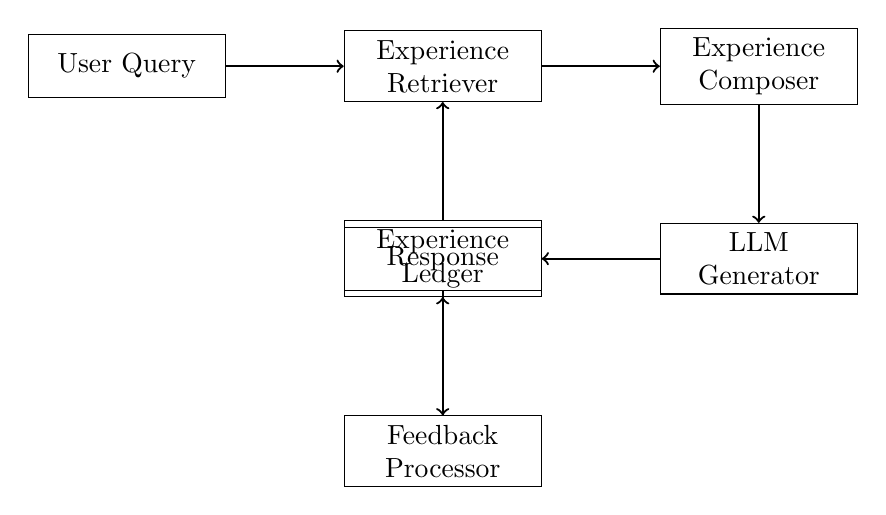
\begin{tikzpicture}[
    node distance=1.5cm,
    box/.style={rectangle, draw, minimum width=2.5cm, minimum height=0.8cm, align=center},
    arrow/.style={->, thick}
]
    \node[box] (input) {User Query};
    \node[box, right=of input] (retriever) {Experience\\Retriever};
    \node[box, right=of retriever] (composer) {Experience\\Composer};
    \node[box, below=of composer] (generator) {LLM\\Generator};
    \node[box, left=of generator] (output) {Response};
    \node[box, below=of retriever] (ledger) {Experience\\Ledger};
    \node[box, below=of ledger] (feedback) {Feedback\\Processor};

    \draw[arrow] (input) -- (retriever);
    \draw[arrow] (retriever) -- (composer);
    \draw[arrow] (composer) -- (generator);
    \draw[arrow] (generator) -- (output);
    \draw[arrow] (ledger) -- (retriever);
    \draw[arrow] (output) -- (feedback);
    \draw[arrow] (feedback) -- (ledger);
\end{tikzpicture}
\caption{Experience Ledger system architecture showing the retrieval-composition-generation pipeline with feedback loop.}
\label{fig:architecture}
\end{figure}

\section{Evaluation}
\label{sec:evaluation}

\subsection{Experimental Setup}

We evaluate Experience Ledgers across three dimensions:

\begin{itemize}
    \item \textbf{Task Success Rate}: First-attempt success on held-out tasks
    \item \textbf{Interaction Efficiency}: Turns required to complete tasks
    \item \textbf{Transfer Effectiveness}: Performance gains from cross-user experiences
\end{itemize}

\subsubsection{Dataset}

We collected 50,000 human-AI interactions across:
\begin{itemize}
    \item Programming assistance (20,000 interactions)
    \item Writing and editing (15,000 interactions)
    \item Data analysis (10,000 interactions)
    \item General Q\&A (5,000 interactions)
\end{itemize}

\subsubsection{Baselines}

We compare against:
\begin{itemize}
    \item \textbf{No Memory}: Standard LLM without retrieval
    \item \textbf{Conversation Cache}: Raw conversation retrieval
    \item \textbf{Summary Memory}: LLM-generated summaries
    \item \textbf{RAG-Documents}: Traditional document retrieval
\end{itemize}

\subsection{Results}

\begin{table}[h]
\centering
\caption{Task success rate comparison across domains}
\label{tab:success}
\begin{tabular}{lcccc}
\toprule
\textbf{Method} & \textbf{Programming} & \textbf{Writing} & \textbf{Analysis} & \textbf{Average} \\
\midrule
No Memory & 0.52 & 0.61 & 0.48 & 0.54 \\
Conversation Cache & 0.58 & 0.64 & 0.53 & 0.58 \\
Summary Memory & 0.61 & 0.67 & 0.56 & 0.61 \\
RAG-Documents & 0.63 & 0.65 & 0.59 & 0.62 \\
\textbf{Experience Ledger} & \textbf{0.71} & \textbf{0.74} & \textbf{0.69} & \textbf{0.72} \\
\bottomrule
\end{tabular}
\end{table}

Experience Ledgers achieve 34\% relative improvement over the no-memory baseline and 16\% improvement over the best baseline (RAG-Documents).

\begin{table}[h]
\centering
\caption{Interaction efficiency (average turns to completion)}
\label{tab:efficiency}
\begin{tabular}{lcccc}
\toprule
\textbf{Method} & \textbf{Programming} & \textbf{Writing} & \textbf{Analysis} & \textbf{Average} \\
\midrule
No Memory & 5.2 & 4.1 & 6.3 & 5.2 \\
Conversation Cache & 4.7 & 3.8 & 5.6 & 4.7 \\
Summary Memory & 4.3 & 3.5 & 5.1 & 4.3 \\
RAG-Documents & 4.1 & 3.4 & 4.8 & 4.1 \\
\textbf{Experience Ledger} & \textbf{2.9} & \textbf{2.4} & \textbf{3.2} & \textbf{2.8} \\
\bottomrule
\end{tabular}
\end{table}

Experience Ledgers reduce interaction turns by 47\% compared to no-memory baseline.

\subsection{Ablation Studies}

\subsubsection{Component Analysis}

\begin{table}[h]
\centering
\caption{Ablation study on Experience Ledger components}
\label{tab:ablation}
\begin{tabular}{lcc}
\toprule
\textbf{Configuration} & \textbf{Success Rate} & \textbf{Avg Turns} \\
\midrule
Full System & 0.72 & 2.8 \\
$-$ Quality Weighting & 0.67 & 3.4 \\
$-$ Experience Composition & 0.68 & 3.1 \\
$-$ Reasoning Traces & 0.64 & 3.6 \\
$-$ Human Feedback & 0.69 & 3.2 \\
\bottomrule
\end{tabular}
\end{table}

Reasoning traces provide the largest contribution, confirming the importance of procedural knowledge.

\subsection{Transfer Learning Analysis}

Cross-user transfer provides 18\% improvement for new users with no prior interactions, demonstrating effective knowledge sharing while preserving privacy.

\section{Related Work}

\textbf{Memory-Augmented Neural Networks}: Work on differentiable memory architectures provides theoretical foundations for persistent memory, though operating at the parameter level rather than instance level.

\textbf{Case-Based Reasoning}: Experience Ledgers draw inspiration from case-based reasoning systems, extending them with neural retrieval and composition.

\textbf{Knowledge Graphs}: While knowledge graphs capture factual knowledge, Experience Ledgers capture procedural knowledge---how to solve problems rather than what is true.

\section{Conclusion}

Experience Ledgers represent a fundamental shift in how AI systems learn from interaction. By capturing and retrieving successful reasoning patterns, we enable AI systems to improve over time without retraining. Our experimental results demonstrate substantial improvements in task success and efficiency, with effective transfer across users and sessions.

Future work will explore federated experience sharing across organizations and integration with continuous learning systems.

\section*{Acknowledgments}

We thank the Zoo community for valuable feedback and the Hanzo engineering team for infrastructure support.

\bibliographystyle{plain}
\begin{thebibliography}{10}

\bibitem{lewis2020rag}
P. Lewis et al., ``Retrieval-Augmented Generation for Knowledge-Intensive NLP Tasks,'' NeurIPS 2020.

\bibitem{graves2014ntm}
A. Graves et al., ``Neural Turing Machines,'' arXiv preprint arXiv:1410.5401, 2014.

\bibitem{ouyang2022rlhf}
L. Ouyang et al., ``Training language models to follow instructions with human feedback,'' NeurIPS 2022.

\bibitem{kolodner1993cbr}
J. Kolodner, ``Case-Based Reasoning,'' Morgan Kaufmann, 1993.

\end{thebibliography}

\end{document}
